%%%
%% This is file `sample-sigplan.tex',
%% generated with the docstrip utility.
%%
%% The original source files were:
%%
%% samples.dtx  (with options: `sigplan')
%%
%% IMPORTANT NOTICE:
%%
%% For the copyright see the source file.
%%
%% Any modified versions of this file must be renamed
%% with new filenames distinct from sample-sigplan.tex.
%%
%% For distribution of the original source see the terms
%% for copying and modification in the file samples.dtx.
%%
%% This generated file may be distributed as long as the
%% original source files, as listed above, are part of the
%% same distribution. (The sources need not necessarily be
%% in the same archive or directory.)
%%
%%
%% Commands for TeXCount
%TC:macro \cite [option:text,text]
%TC:macro \citep [option:text,text]
%TC:macro \citet [option:text,text]
%TC:envir table 0 1
%TC:envir table* 0 1
%TC:envir tabular [ignore] word
%TC:envir displaymath 0 word
%TC:envir math 0 word
%TC:envir comment 0 0
%%
%%
%% The first command in your LaTeX source must be the \documentclass command.
%%\documentclass[sigplan,nonacm]{acmart}
\documentclass[sigplan, nonacm]{acmart}\settopmatter{printfolios=true,printccs=false,printacmref=false}

\graphicspath{{pictures/}}
%%
%% \BibTeX command to typeset BibTeX logo in the docs
\AtBeginDocument{%
	\providecommand\BibTeX{{%
			\normalfont B\kern-0.5em{\scshape i\kern-0.25em b}\kern-0.8em\TeX}}}

%% Rights management information.  This information is sent to you
%% when you complete the rights form.  These commands have SAMPLE
%% values in them; it is your responsibility as an author to replace
%% the commands and values with those provided to you when you
%% complete the rights form.
%%\setcopyright{acmcopyright}
\setcopyright{none}
%%\acmJournal{PACMPL}
%%\acmVolume{1}
%%\acmNumber{CONF} % CONF = POPL or ICFP or OOPSLA
%%\acmArticle{1}
%%\acmYear{2021}
%%\acmMonth{9}
%%\acmDOI{}
%%\copyrightyear{2018}
%%\acmYear{2018}
%%\acmDOI{10.1145/1122445.1122456}

%% These commands are for a PROCEEDINGS abstract or paper.
%%\acmConference[Woodstock '18]{Woodstock '18: ACM Symposium%% on Neural
%%  Gaze Detection}{June 03--05, 2018}{Woodstock, NY}
%%\acmBooktitle{Woodstock '18: ACM Symposium on Neural Gaze Detection,
%%  June 03--05, 2018, Woodstock, NY}
%%\acmPrice{15.00}
%%\acmISBN{978-1-4503-XXXX-X/18/06}


%%
%% Submission ID.
%% Use this when submitting an article to a sponsored event. You'll
%% receive a unique submission ID from the organizers
%% of the event, and this ID should be used as the parameter to this command.
%%\acmSubmissionID{123-A56-BU3}

%%
%% The majority of ACM publications use numbered citations and
%% references.  The command \citestyle{authoryear} switches to the
%% "author year" style.
%%
%% If you are preparing content for an event
%% sponsored by ACM SIGGRAPH, you must use the "author year" style of
%% citations and references.
%% Uncommenting
%% the next command will enable that style.
%%\citestyle{acmauthoryear}
\usepackage{xspace}
\usepackage{booktabs}   %% For formal tables:
                        %% http://ctan.org/pkg/booktabs
\usepackage{subcaption} %% For complex figures with subfigures/subcaptions
                        %% http://ctan.org/pkg/subcaption

\usepackage[utf8]{inputenc}
\usepackage[T1]{fontenc}
\usepackage[scaled=0.78]{beramono}
\usepackage{amsmath}
\usepackage{mathtools}
\usepackage{stmaryrd}
%\usepackage{unicode-math}
%\usepackage{MnSymbol}
\usepackage{wasysym}
\usepackage{color}
\usepackage{xcolor,colortbl}
\usepackage{url}
\usepackage{listings}
\usepackage{paralist}
%\usepackage[compact]{titlesec}
\usepackage[font={small}]{caption}
\usepackage{wrapfig}
\usepackage{enumitem}
\usepackage{multicol}
\usepackage{multirow}
\usepackage{makecell}
\usepackage{flushend}
\usepackage{bcprules}
\usepackage{textcomp}
\usepackage{tikz}
\usetikzlibrary{positioning,fit,calc,arrows.meta,arrows,decorations}
\usepackage{pdfpages}
\usepackage{cleveref}
\usetikzlibrary{matrix}
\usepackage{xspace}
\definecolor{light-gray}{gray}{0.85}
\usepackage{stackengine}
\usepackage{mathpartir}
% ----- listings

%\definecolor{ckeyword}{HTML}{7F0055}
\definecolor{ckeyword}{HTML}{000000}
\definecolor{ccomment}{HTML}{3F7F5F}
\definecolor{cstring}{HTML}{2A0099}

\lstdefinelanguage{Scala}%
{morekeywords={
  abstract, sealed, lazy,
  case,catch,char,class,%
  def,do,else,extends,final,finally,for,%
  if,import,implicit,%
  match,module,%
  new,null,undefined,%
  %fun,
  array,
  override,%
  package,private,protected,public,%
  for,public,return,super,%
  this,throw,trait,try,type,%
  val,var,%
  with,while,%
  object,
  let,skip,assert,then,fst,snd,idx,sum,prod,exists,forall,%
  yield,%
  % some scheme keywords
  define, null?, car, cdr
  },%
  sensitive,%
  moredelim=*[il][\bfseries]{\#\#\ },
  morecomment=[l]//,%
  morecomment=[s]{/*}{*/},%
  morestring=[b]",%
  %morestring=[b]',%
  showstringspaces=false%
}[keywords,comments,strings]%

\lstdefinelanguage{Effect}%
{morekeywords={
    effect, yield, return
  },%
  sensitive,%
  moredelim=*[il][\bfseries]{\#\#\ },
  morecomment=[l]//,%
  morecomment=[s]{/*}{*/},%
  morestring=[b]",%
  %morestring=[b]',%
  showstringspaces=false%
}[keywords,comments,strings]%

\lstdefinelanguage{LLVM}%
{morekeywords={
    define, i32, br, icmp, sub, call, mul, phi, ret, label
  },%
  sensitive,%
  moredelim=*[il][\bfseries]{\#\#\ },
  morecomment=[l];,%
  morecomment=[s]{/*}{*/},%
  morestring=[b]",%
  %morestring=[b]',%
  showstringspaces=false%
}[keywords,comments,strings]%

\lstdefinelanguage{CPP}%
{morekeywords={
    using, void, function, if, else, Cont, List
  },%
  sensitive,%
  moredelim=*[il][\bfseries]{\#\#\ },
  morecomment=[l]//,%
  morecomment=[s]{/*}{*/},%
  morestring=[b]",%
  %morestring=[b]',%
  showstringspaces=false%
}[keywords,comments,strings]%


\lstset{
  language=Scala,%
  mathescape=true,%
%  columns=[c]fixed,%
  aboveskip=2pt,%\smallskipamount,
  belowskip=1pt,%\negsmallskipamount,
  lineskip=-1pt,
  basewidth={0.6em, 0.5em},%
%  backgroundcolor=\color{listingbg},
  basicstyle=\ttfamily,
  keywordstyle=\keywordstyle,
  commentstyle=\commentstyle,
  stringstyle=\stringstyle,
%  xleftmargin=0.5cm
  literate={-->}{{$\to$}}2
           {->}{{$\mapsto$}}3
           {<-}{{$\leftarrow$}}2
           {=>}{{$\Rightarrow ~$}}2
           {|-}{{$\ts$}}2
           %{fun}{{$\lambda$}}1
           {idx}{{$\#$}}1
           {array(}{{$\langle.\rangle$(}}3
           {σ}{{$\sigma$}}1
           {ρ}{{$\rho$}}1
           {→}{{$\to$}}1
           {←}{{$\leftarrow$}}1
           {λ}{{$\lambda$}}1
           {α}{{$\alpha$}}1
           {⊔}{{$\sqcup$}}1
           {⊓}{{$\sqcap$}}1
           {⊑}{{$\sqsubseteq$}}1
           {⊤}{{$\top$}}1
           {⊥}{{$\bot$}}1
           {×}{{$\times$}}1
           {τ}{{$\tau$}}1
           {ψ}{{$\psi$}}1
           {Σ}{{$\Sigma$}}1
           {⟨}{{$\langle$}}1
           {⟩}{{$\rangle$}}1
           {π}{{$\pi$}}1
           {∪}{{$\cup$}}2
           %{[[}{{$[\![$}}1
           %{]]}{{$]\!]$}}1
           %{…}{{$\!...$}}1
}

\lstdefinestyle{small}{
  language=Scala,%
  mathescape=true,%
%  columns=[c]fixed,%
  aboveskip=2pt,%\smallskipamount,
  belowskip=1pt,%\negsmallskipamount,
  lineskip=-1pt,
  basewidth={0.6em, 0.45em},%
%  backgroundcolor=\color{listingbg},
  basicstyle=\fontsize{7}{9}\selectfont\ttfamily,
  keywordstyle=\keywordstyle,
  commentstyle=\commentstyle,
  stringstyle=\stringstyle,
%  xleftmargin=0.5cm
  literate={-->}{{$\to$}}3
           {->}{{$\mapsto$}}3
           {=>}{{$\Rightarrow ~$}}2
           {|-}{{$\ts$}}2
           %{fun}{{$\lambda$}}1
           {idx}{{$\#$}}1
           {sum}{{$\Sigma$}}1
           {array(}{{$\langle.\rangle$(}}3
           {σ}{{$\sigma$}}1
           {ρ}{{$\rho$}}1
           {→}{{$\to$}}1
           {λ}{{$\lambda$}}1
           {α}{{$\alpha$}}1
           {⊔}{{$\sqcup$}}1
           {⊓}{{$\sqcap$}}1
           {⊑}{{$\sqsubseteq$}}1
           {⊤}{{$\top$}}1
           {⊥}{{$\bot$}}1
           {×}{{$\times$}}1
           {τ}{{$\tau$}}1
           {ψ}{{$\psi$}}1
           %{[[}{{$[\![$}}1
           %{]]}{{$]\!]$}}1
           %{…}{{$\!...$}}1
}

\lstdefinestyle{extrasmall}{
  language=Scala,%
  mathescape=true,%
%  columns=[c]fixed,%
  aboveskip=2pt,%\smallskipamount,
  belowskip=1pt,%\negsmallskipamount,
  lineskip=-1pt,
  basewidth={0.6em, 0.45em},%
%  backgroundcolor=\color{listingbg},
  basicstyle=\fontsize{6}{8}\selectfont\ttfamily,
  keywordstyle=\keywordstyle,
  commentstyle=\commentstyle,
  stringstyle=\stringstyle,
%  xleftmargin=0.5cm
  literate={-->}{{$\to$}}3
           {->}{{$\mapsto$}}3
           {=>}{{$\Rightarrow ~$}}2
           {|-}{{$\ts$}}2
           %{fun}{{$\lambda$}}1
           {idx}{{$\#$}}1
           {sum}{{$\Sigma$}}1
           {array(}{{$\langle.\rangle$(}}3
           {σ}{{$\sigma$}}1
           {ρ}{{$\rho$}}1
           {→}{{$\to$}}1
           {λ}{{$\lambda$}}1
           {α}{{$\alpha$}}1
           {⊔}{{$\sqcup$}}1
           {⊓}{{$\sqcap$}}1
           {⊑}{{$\sqsubseteq$}}1
           {⊤}{{$\top$}}1
           {⊥}{{$\bot$}}1
           {×}{{$\times$}}1
           %{[[}{{$[\![$}}1
           %{]]}{{$]\!]$}}1
           %{…}{{$\!...$}}1
}

\definecolor{listingbg}{RGB}{240, 240, 240}

\newcommand{\commentstyle}[1]{\color{ccomment}\itshape{#1}}
\newcommand{\keywordstyle}[1]{\color{ckeyword}\bfseries{#1}}
%\newcommand{\keywordstyle}[1]{\color{ckeyword}{#1}}
%\newcommand{\stringstyle}[1]{\color{cstring}\bfseries{#1}}
\newcommand{\stringstyle}[1]{\color{cstring}\text{#1}}

\lstnewenvironment{listing}{\lstset{language=Scala}}{}
\lstnewenvironment{listingtiny}{\lstset{language=Scala,basicstyle=\scriptsize\ttfamily}}{}

\newcommand{\code}[1]{\lstinline[language=Scala,columns=fixed,basicstyle=\ttfamily]|#1|}

% ----- packed items, so we don't waste space
\newenvironment{sitemize}{
\begin{itemize}[leftmargin=2.5ex]
  \setlength{\itemsep}{1pt}
  \setlength{\parskip}{0pt}
  \setlength{\parsep}{0pt}
}{\end{itemize}}

\newenvironment{senumerate}{
\begin{enumerate}[leftmargin=2.5ex]
  \setlength{\itemsep}{1pt}
  \setlength{\parskip}{0pt}
  \setlength{\parsep}{0pt}
}{\end{enumerate}}

\newcommand{\mypar}[1]{{\bf #1.}}

% ----- formal

%\newcommand{\judgement}[2]{{\bf #1} \hfill #2}
%\newcommand{\den}[1]{$\left\llbracket$\;#1\;$\right\rrbracket$}
\newcommand{\den}[1]{\llbracket~#1~\rrbracket}

%\newcommand{\ts}{\,\vdash\,}
\newcommand{\evalsto}{\Downarrow}

\newcommand{\mbind}{\;{\small{\texttt{>>}\hspace{-0.3pt}\raisebox{-0.15pt}{\texttt{=}}}}\;}

%\newcommand{\mbind}{{\small{\texttt{>>}\hspace{-1.7pt}\raisebox{-0.15pt}{\texttt{=}}}}}

\newcommand{\rref}[1]{\textsc{(#1)}}

% ----- comments and todo

\newcommand{\note}[1]{{\color{red}[#1]}}
\newcommand{\snote}[1]{{\color{blue}[#1]}}
\newcommand{\todo}[1]{\note{TODO: #1}}
\newcommand{\rev}[1]{\note{Revision: #1}}

\newcommand{\silent}[1]{}

\newcommand{\hl}[1]{\setlength{\fboxsep}{0pt}\colorbox{light-gray}{#1}}

%\newcommand{\SECFork}{\textsc{sec}$_{\pitchfork}$}
\newcommand{\SECFork}{\textsc{sec}$_{{\mathrlap{<}-}}$}
\newcommand{\SECConc}{\textsc{sec}$_v$}
\newcommand{\SECBack}{\textsc{sec}$_{\hookleftarrow}$}



%%
%% end of the preamble, start of the body of the document source.
\newcommand{\tool}{\textsc{GenSym}\xspace}
\newcommand{\ul}[1]{\underline{#1}}
\newcommand{\lb}{\{~}
\newcommand{\rb}{~\}}

\newcommand{\Typ}[1]{\ensuremath{\mathsf{#1}}}
\newcommand{\Ast}[1]{\ensuremath{\textsf{\text{#1}}}}
\newcommand{\Def}[1]{\ensuremath{\mathrm{#1}}}
\newcommand{\mit}[1]{\ensuremath{\mathit{#1}}}
\newcommand{\msf}[1]{\ensuremath{\mathsf{#1}}}

\newcommand{\lang}{\textsf{SimpLLVM}\xspace}

\newcommand{\Sem}[3][]{\ensuremath{\llbracket {#2} \rrbracket_{#3}^{#1}}}
\newcommand{\SSem}[2]{\ensuremath{\llbracket {#1} \rrbracket_{#2}^{\#}}}
\newcommand{\State}{\mathbb{S}}
\newcommand{\Address}{\mathcal{A}}
\newcommand{\Mem}{\mathbb{M}}
\newcommand{\Value}{\mathcal{V}}
\newcommand{\Loc}{\msf{Loc}}
\begin{document}
\sloppy

%%
%% The "title" command has an optional parameter,
%% allowing the author to define a "short title" to be used in page headers.
\title{Environment modeling in \tool}

%%
%% The "author" command and its associated commands are used to define
%% the authors and their affiliations.
%% Of note is the shared affiliation of the first two authors, and the
%% "authornote" and "authornotemark" commands
%% used to denote shared contribution to the research.
\author{Ruiqi Gao}
\email{gao606@purdue.edu}
\affiliation{%
  \institution{Purdue University}
  \city{Lafayette}
  \state{Indiana}
  \country{USA}
  \postcode{47901}
}

\begin{abstract}
  Symbolic execution is a popular program analysis technique for software security and verification. It aims to explore multiple feasible execution of a program in parallel while gathering the corresponding path constraints. As real-world programs often require interaction with the underlying operating system, modeling the environment plays a crucial role in symbolic execution. Coreutils is a collection of the basic file, shell manipulation commands of the GNU operating system. It is used by most symbolic execution framework as a stress test benchmark for intense environment interactions. \par
  \tool is a symbolic execution compiler for LLVM IR that realizes efficient execution by compilation. In this paper, we first present two different approaches of environment modeling for \tool. Then we demonstrate various obstacles we overcome towards testing Coreutils in \tool. Finally we compare our framework with other symbolic engine based on benchmarks of Coreutils.

\end{abstract}

\keywords{Symbolic Execution, Environment Modeling, \tool, Coreutils}

\maketitle
\section{Introduction}
Symbolic execution is widely used in software verification, bug-finding and automatic test generation. Although traditional unit testing is sufficient for most scenarios, it is still a under-approximation due to its inherent nature and requires increasing maintenance as program develops. First introduced in the 1970s\cite{boyer1975select, howden1977symbolic, king1975new, king1976symbolic}, symbolic execution can simultaneously explore different execution paths by making certain input symbolic and accompanying each path with a state. A state in symbolic execution engine is composed of 2 parts, a set of boolean formula to describe the path condition and a symbolic store that map variables to both symbolic and concrete values. Execution within a basic block will update the symbolic store the same as   the corresponding native execution. The executing path will fork when a branch with symbolic condition is encountered, generate two paths represent the true and false branch, check their feasibility with solver and update path condition accordingly. With the development of SMT\cite{barrett2021satisfiability} solvers like Z3\cite{moura2008z3}, symbolic execution is becoming increasingly practical and efficient.\par
\subsection{\tool}
Traditional symbolic execution engine like KLEE\cite{cadar2008klee} is interpreter-based. The interpreter will traverse the compiled intermediate representation (IR) of the program, mapping each instruction into its symbolic semantic and update the path condition and symbolic store within their customized state representation according to the strategy we described above. Although interpreter-based symbolic execution can detect all potential bugs in theory, problems like path-explosion \cite{baldoni2018survey} prevent it from scaling up to large programs. The interpretation overhead of translating instruction into its symbolic semantic will also cause a significant performance slow-down.\par
Another approach to implement symbolic execution is instrumentation\cite{10.1145/1180405.1180445, CREST}. Instrumentation does not require a internal state-representation and avoid the interpretation overhead. Instructions on concrete values is executed natively while execution on symbolic values is achieved through instrumented code. Instrumentation naturally works well with concolic execution \cite{godefroid2005dart, sen2005cute} where only a single path is reasoned about at a time. While instrumentation achieves better performance compared to interpretation, its lack of state-representation prevents it from adopting certain optimization like state-merging and path selection strategies. \par
\tool is the first symbolic execution compiler framework that adapts compiler and code generation technique for symbolic execution. It eliminates the overhead of Interpretation while give user fine-grained control over the state representation, and achieves flexible and efficient symbolic execution. Various optimization and heuristic can be easily adopted in \tool by inspecting and manipulation over the internal state and control representation. The core idea of \tool is to specialize a symbolic interpreter with the input program using Partial evaluation\cite{damian1999partial}. According to the first Futamura projection\cite{Futamura1971, Futamura1999}, the specialized program is equivalent to running the interpreter with the input code. \tool achieves partial evaluation for the symbolic interpreter using staging\cite{DBLP:conf/pepm/TahaS97} and avoid the need to manually developing a complex specializer. With the symbolic interpreter annotated with stages, the program can be easily specialized using meta-programming, and we can get a symbolic execution compiler for free. Based on LMS\cite{rompf2010lightweight} - a library-based staging compiler that distinguishes stages solely on Type, \tool specializes a staged symbolic interpreter into a compiler and eliminates the interpretation overhead.
\subsection{Environment Modeling}
As most programs are not self-contained, they need to interact with the underlying environment (operating system, network). Different flavors of symbolic execution have different treatment for external calls. \par
Instrumentation based concolic execution can directly invoke the native external call as each path is executed concretely. This approach is simple and straightforward but sacrifice the completeness of exploration. An alternative approach is to create an abstract model of environment accompanying different execution paths. As modeling external call at the library level is expensive, most framework chooses to model the environment at the system call level.
 KLEE\cite{cadar2008klee} develops a core symbolic file system where different paths can invoke system call in isolation. \par
The approaches above only investigates which part of the environment should be modeled but neglect the question about how to model the environment. As we mentioned above, \tool is a symbolic execution compiler that translate the programs in Source Language S to programs in Target language T. Intuitively, we can choose to model the environment in both the Source Language level (as part of the user program) and the Target Language level (as runtime library). Like KLEE, we choose to model the environment in the system call level with a symbolic file system. Using the flexibility of our framework, we can choose between directly poring KLEE' file system or developing a internal file system in the backend.\par
Coreutils \cite{coreutilsweb} is a collection of commonly used GNU command that manipulate file system, shell and text. It interacts intensively with the operating system and is used by most symbolic execution framework as benchmarks. We also use Coreutils as a stress test and benchmark for our environment modeling implementation.
\subsection{Paper Structure}
The paper is organized as follows: \par \par
In section \ref{twofsimpl}, we will discuss and compare two file system implementations (in the source language level and target language level).\par
In section \ref{coreutilstests}, we will discuss various obstacles and performance bottlenecks we observed in  adapting Coreutils tests into our engine and our corresponding solutions.\par
In section \ref{evaluation}, we present benchmarks of Coreutils programs in our engine with two file system implementations and KLEE.\par
In section \ref{conclusion}, we summarize our work and draw some conclusions.

\section{Different levels of Environment Modeling}\label{twofsimpl}
In the context of symbolic execution compiler, we can choose between modeling the environment in the source language level or in the target language level. \tool translates LLVM-IR (compiled from C programs) into backend C++ programs. As we mentioned before, we choose to model the environment in the file system level like KLEE, so we can either directly porting KLEE's file system (written in C) or develops our own internal file system as backend C++ runtime library. We will discuss this two implementations in detail and compare their advantage and disadvantage.
\paragraph*{Porting KLEE's file system}
KLEE develops a POSIX-like symbolic file system on top of the native file system in order to alleviate side effects caused by external calls and prevent interference across execution paths. The symbolic file system is written purely in C and can be linked with the user program to be analyzed. This file system can be easily modified and extended without mangling
 with the internal details. In fact, by implementing the entire symbolic file system in the C level, it can be ported to other well-formed symbolic engine with no modification. We can directly port KLEE's file system into our model with little effort.\par
 KLEE's file system is a hybrid approach, it contains both symbolic files and concrete files. It maintains symbolic meta data like offset and open flags for both symbolic and concrete files. For symbolic files, it will allocated a char array buffer upon creation to store its symbolic content and a symbolic stat struct to store its symbolic status. For concrete file, it will records its actual file descriptor upon open for future references.\par
\begin{figure}[t]
\centering
\begin{subfigure}{0.5\textwidth}
\begin{lstlisting}[style=small,language=C,numbers=left,stepnumber=1,xleftmargin=2em,numberstyle=\ttfamily]
ssize_t write(int fd, const void *buf, size_t count) {
  exe_file_t *f;
  f = get_file(fd);

  if (is_concrete_file(f)) {
    /* concrete file, directly invoke corresponding native syscall */
    int r = syscall(__NR_pwrite64, f$\rightarrow$fd, buf, count, (off64_t) f$\rightarrow$off);

    f$\rightarrow$off += r;
    return r;
  } else {
    /* symbolic file, copy the symbolic data from buf into current
     file's buffer */
    size_t actual_count = min(count, f$\rightarrow$dfile->size - f$\rightarrow$off);

    memcpy(f$\rightarrow$dfile$\rightarrow$contents + f$\rightarrow$off, buf, actual_count);

    f$\rightarrow$off += actual_count;
    return actual_count;
  }
}
\end{lstlisting}
\vspace{-1em}
%\caption{The generated code of the LLVM \texttt{power} function by \tool.
\end{subfigure}
\caption{
  Upper: The sketch of KLEE file system's write() }
\vspace{-0.3in}
\label{fig:example}
\end{figure}

 Each system call interacting with the file system will check whether the file is a symbolic file first as shown in Figure \ref{fig:example}. If the file is symbolic, it will use memcpy or other memory modification function to manipulate the char array buffer storing the actual symbolic content. If the file is concrete, it will uses the stored actual file descriptor to access the real file stored on disk. KLEE's file system stores offset for both symbolic and concrete files and uses pread() and pwrite() to accessing concrete files using the managed offset to prevent interference between paths.\par
 KLEE's file system is a simple and straightforward approach to model the environment in the source language level, it can switch between invoke native system call and access internal symbolic file system. We directly reuse it as the source language implementation of the file system.
 \paragraph*{Implementing File system as Runtime Library}
Besides modeling the file system in the source language level, we can also develop a symbolic file system in the target language as runtime libraries. By embedding the file system inside the state, file system operations can be viewed as operating on the file system object.
$$ \State = \langle \msf{Heap} \times \msf{Stack} \times \msf{PC} \times \msf{Label} \times \msf{FS} \rangle $$
We can also specify the signature of primitive operations of \msf{FS}, e.g.:
$$ \msf{open} : \msf{FS} \times \msf{String} \times \msf{Mode} \to \msf{FS} \times \mathbb{N}$$
$$ \msf{read} : \msf{FS} \times \msf{Fd} \times \msf{Address} \times \mathbb{N} \to \msf{FS} \times \mathbb{N}$$
$$ \msf{write} : \msf{FS} \times \msf{Fd} \times \msf{Address} \times \mathbb{N} \to \msf{FS} \times \mathbb{N}$$
With knowledge of the detailed internal memory model and state representation, we can write more optimized code of each file system operations for different engines.\par
Besides directly writing the file system in the target language (C++) level, we can also use meta programming and code generation techniques to generate the file system library in LMS.
\subsection*{Comparison between the two approaches}
Implementing the file system in the source language level has the advantages of portability and flexibility. It can be ported to a completely different framework with little effort without the need to mangle with the underlying internal engine details. We can also switch more flexibly  between different designs. For example, we can enable symbolic filenames simply by making the filename symbolic and requires no modification in the file system, the underlying symbolic engine will deal with the state forking as it analyzes our file system code along with the user code after linking. However, in order to achieve the same goal in the target language level implementation, we will need to understand the internal control representation (direct style or CPS-style) and modify the open system call in the runtime library to handle the possible forking of states accordingly.\par
Although implementing file system in the source language is portable and flexible, it lacks efficiency and performance. As a example, we can look at the write() system call implementation sketch in Figure \ref{fig:example}. All the control flow structure (if-else statement, function call) will be compiled into the corresponding backend control representation, increasing the performance overhead. Furthermore, if we are accessing a symbolic file, write() will invoke memcpy function, triggering a loop to copy the memory. Inside each loop iterations, memcpy will first use lookup to read one byte from the src address, and then write the byte into the dest address. Because the file system is implemented on the source language level, each memory read and write will be compiled into lookup and update of internal memory model and invoke the corresponding runtime library, causing significant performance degrading. The source language level file system always executes on top of the underlying control and memory representation, resulting multiple levels of indirection and slow down the overall performance. We can see more concrete examples in the benchmark in section \ref{evaluation}.
\section{Testing Coreutils}\label{coreutilstests}
Coreutils is a good test suite for evaluating symbolic execution in the aspect of environment modeling as it contains commonly used linux commands that interact intensively with  the operating system. Coreutils contains 89 programs and more than 80000 lines of code in total. Coreutils not only test our two file system implementations but also measure the overall robustness and correctness of the entire compiler framework as it contains most commonly used C language features. We have only tested small self-contained programs before, therefore testing Coreutils reveals a lot of hidden problems and performance bottlenecks in our engine.\par
Coreutils programs uses most C language features, some complex usage like complex nested structure with pointer member, conversions between integer and pointer and variable argument lists will trigger bugs in our previous engine, and they have all been fixed accordingly. We also found several missing external functions in the compiled IR of Coreutils programs, they are also added in our current implementation. Besides the correctness problem found during testing of Coreutils programs, a major performance bottlenecks was also found - the compilation time overhead.
\subsection{Compilation time optimization}
We need to link the Coreutils program with the uClibc \cite{uclibcweb} standard library because we only model the environment in the system call level. After linking, the final complete user program is very large and will take a non-negligible long compilation time. For example, echo can take up to 10 minutes to compile into the final executable file. Most Coreutils programs do not vary much in code size, so the observed compilation time overhead is indeed a bottleneck towards achieving fast iteration over the testing-debugging process and prevent us from testing more Coreutils programs quickly. After profiling, we are able to identify the main causes for the compilation time overhead and address them accordingly. The compilation time bottleneck can be divided into two aspects, Scala part and C++ part:
\paragraph*{Scala part compilation}
\tool is based on LMS framework which is written in Scala, as a result the core stage interpreter and the backend code generator are both written in Scala. The overhead in the Scala part compilation is a result of both the large size of the fully linked program and the large locale of type $struct \quad \_ \_ locale \_ mmap \_ t$ in uClibc library. After linking with both the uClibc library and KLEE's file system, the final analyzed program of echo contains 28947 lines of LLVM-IR and a large locale structure of 274282 bytes. To make the situation worse, LMS realizes meta programming through overloading of the second stage operation, and the second stage operations will finally generate internal IR nodes and the whole staged program is translated into a graph of IR nodes. The compiled graph of the fully linked echo programs contains 460263 nodes and will trigger lots of hidden problems because we have not test graph of this kind of large size before. \par
LMS framework uses Sea of Nodes IR where Nodes are connected through data and effect dependencies edges. Most of the non-local optimization in LMS relies on traversing through the IR nodes to gather certain information required for analysis. We observe a severe performance degrading in DeadCodeElimination optimization for code generation caused by badly selected data structures. The DeadCodeElimination optimization needs to collect the live and reachable set of symbols in order to find out the dead nodes. This optimization uses HashSet to store the live and reachable symbols. This optimization will frequently update the two HashSet, and cause frequent hashing and rehashing due to collision. Given the large size of nodes in the generated graph, the frequent collision will significantly slow down the analysis procedure. As a result, it could not finish this single optimization even for over one and a half hour. However, this bottleneck can be easily avoided due to the fact that our internal IR like most modern IR is of SSA form, each symbol is annotated with a unique number, then instead of using HashSet to store all symbols, we can directly use BitSet to store the identification number of each symbol and avoids hashing. This solution resolves the performance degrading and the optimization can finish in less than two seconds as a result.\par
Another compilation time overhead is caused by the dynamic scheduling in certain analysis pass. Because LMS uses a Sea of Nodes IR, each IR node is not statically assigned to blocks, instead the nodes are connected through data and effect dependencies and can move freely as long as it does not violate the dependencies. The base class of analyzer in LMS is a traverser and it will dynamic schedule the sea of nodes IR every time to calculate the IR of each blocks. For large scale graph, dynamic scheduling actually takes up most time of the analysis and optimization. As a case study, we can look at the AssignElimination optimization pass where we try to eliminate unused local stack variables. This pass consists a traverser to filter out the unused stack variable and a transformer to rebuild the optimized graph. This optimization needs to schedule the graph twice because both traverser and transformer will schedule the graph. As a result, the whole optimization takes about 70s for echo program while 60s of it is spent on the scheduling. However, we can perform the optimization without the need to schedule the whole graph in the analysis traverser. After rewriting the analysis procedure, we can reduce the entire optimization time to 40s. \par
Apart from the two overhead caused by the large code size of the linked Coreutils problem, a different sort of compilation time bottleneck is found caused by the large locale structure in uClibc code. As we mentioned above, the large locale structure in uClibc takes 274282 bytes in total. After compilation, the locale is translated into a large list of the same size. A large amount of overhead is caused by ill treatment for large list in the Scala code. Our engine pre-process the global data as a preheap and put it in front of the actual symbolic heap in a large vector. Our preheap processing code uses foldleft to evaluate the global variable of struct and array type, and it has poor performance especially when dealing with large list. By switching to map, we are able to reduce the preheap processing time considerably. A similar problem is found in the backend C++ code generators. Our engine uses zipWithIndex often in the C++ code generator for List, and zipWithIndex would eagerly generates the resulting zipped list first. It performs poorly when dealing with large list like the large locale structure mentioned above. After rewriting of this common pattern, we are able to greatly reduce the time spent on backend code generator for list.
\paragraph*{C++ part compilation}
\tool generate a C++ file for each function in the analyzed program, this naturally favors multi core compilation. For example, the fully linked echo program will be compiled into 155 C++ files. As a result, it is beneficial to use multi-core processor and exploit parallel compilation. Although most of the file can be compiled very quickly, the compilation of main file will get stuck when optimization is enabled. Our engine will pre-process the global data into a large list and put it in front of the actual heap in a large vector as the initial symbolic heap. Each element of the vector is a pointer into the actually value (concrete or symbolic), created by a corresponding wrapper function. After profile and debug, we observe that the initialization list of the large pre-heap vector will be first allocated on stack, then each element of the vector has to be assigned by calling the corresponding initialization function. The body of the main function is enormous and the optimization will get stuck. Furthermore, a specific optimization pass SROA (replacement of aggregates) will try to split the large stack allocated object into pieces in order to fit them inside registers. This pass will try to analyze the large stack allocated initialization list and stall the entire compilation. This problem is un-avoidable in our current implementation without a complete rewrite of the code generation strategy. We choose to only use O0 to compile the main file and O3 to compile other generated program. This will not affect the overall runtime performance as the main function is a start-up procedure for the entire symbolic execution and is only a one-time effort. We will see some concrete evidence from benchmarks compared to KLEE in Section \ref{evaluation}.
\paragraph*{Compilation time after refactoring}
After diagnose the cause of compilation time overhead in Scala part and C++ part and fix them accordingly, we are able to compile the entire program into executable file in less than two minutes. This is totally acceptable compared to more than 10 minutes in the un-optimized engine. We are able to test more Coreutils programs and achieve fast-iteration over the test-fix-verify procedure.
\section{Evaluation}\label{evaluation}
This section shows the evaluation benchmarks of running Coreutils programs on \tool with both two file systems and KLEE. \tool has two file system implementations, one written in the source language level (directly porting KLEE's POSIX filesystem), one written in the target language level as runtime library. We also run the same program on KLEE to compare the performance with \tool. Because we directly port KLEE's file system as the source level implementation, comparison between \tool with KLEE's POSIX file system and KLEE is fair and can measure the efficiency of this two symbolic execution engines. We will use \tool/POSIX to represent our framework with KLEE's filesystem implementation, \tool/FS to represent our framework with the internal target language level file system implementation and KLEE/POSIX to represent KLEE with its file system. We choose echo from Coreutils programs for testing and we perform all the experiment on the Intel(R) Xeon(R) Platinum 8168 CPU @ 2.70GHz 192 core cpu on server bigdata2.cs.purdue.edu. We use g++ with -O3 to compile the generated C++ code as mentioned in section \ref{coreutilstests}. The running time is shown in Table \ref{tab:coreutils_benchmarks_echo} and Figure \ref{fig:speedup}.\par
%%\begin{table}[h]
%%  \vspace{-0.75em}
%%  \footnotesize
%%\caption{Comparing the running timesof \tool/POSIX, \tool/FS and KLEE/POSIX
%%  using different numbers of symbolic inputs (\#Sym).
%%  ``\#Path'' is the number of paths explored.}
%%  %Speed up indicates the performance gain of \tool/FS over \tool/POSIX.
%%  \vspace{-0.75em}
%%\begin{tabular}{c|cccccc}
%%
%%  \hline
%%                 & \textbf{\#Sym}    & 6     & 7     & 8    & 9     & 10      \\
%%                 & \textbf{\#Path}   & 575     & 1679    & 4971  & 14825  & 44362      \\
%%                 \hline
%%  \textbf{KLEE/POSIX} & \textbf{Time(s)} & 4.52  & 12.17  & 38.20 & 147.54  & 438.99   \\
%%  \textbf{\tool/POSIX} & \textbf{Time(s)}  & 0.78 & 2.28 & 7.32 & 23.25 & 76.08 \\
%%  \textbf{\tool/FS}   & \textbf{Time(s)}  & 0.55 & 1.59 & 5.07 & 16.60  & 54.84  \\
%%                 \hline
%%  \end{tabular}
%%\label{tab:coreutils_benchmarks_echo}
%%\vspace{-1em}
%%\end{table}
\begin{table}[h]
  \vspace{-0.75em}
  \footnotesize
\caption{Comparing the running times of \tool/POSIX, \tool/FS and KLEE/POSIX
  using different numbers of symbolic inputs (\#Sym).
  ``\#Path'' is the number of paths explored.}
  %Speed up indicates the performance gain of \tool/FS over \tool/POSIX.
  \vspace{-0.75em}
\begin{tabular}{c|cccccc}

  \hline
                & \textbf{\#Sym}    & 6     & 7     & 8    & 9     & 10      \\
                & \textbf{\#Path}   & 575     & 1679    & 4971  & 14825  & 44362      \\
                 \hline
  \textbf{KLEE/POSIX} &\textbf{Time(s)} & 4.52  & 12.17  & 38.20 & 147.54  & 438.99   \\
  \textbf{\tool/POSIX}& \textbf{Time(s)}  & 0.78 & 2.28 & 7.32 & 23.25 & 76.08 \\
  \textbf{\tool/FS}   &\textbf{Time(s)}  & 0.55 & 1.59 & 5.07 & 16.60  & 54.84  \\
                 \hline
  \textbf{\tool/POSIX over}   &  \\
  \textbf{KLEE/POSIX}   &\textbf{Speedup}  & 5.79 & 5.34 & 5.22 & 6.35  & 5.77  \\
  \hline
  \textbf{\tool/FS over}   &  \\
  \textbf{\tool/POSIX}   &\textbf{Speedup}  & 1.42 & 1.43 & 1.44 & 1.40  & 1.39  \\
  \hline
  \end{tabular}
\label{tab:coreutils_benchmarks_echo}
\vspace{-1em}
\end{table}
\begin{figure}[htbp]
  \centering
  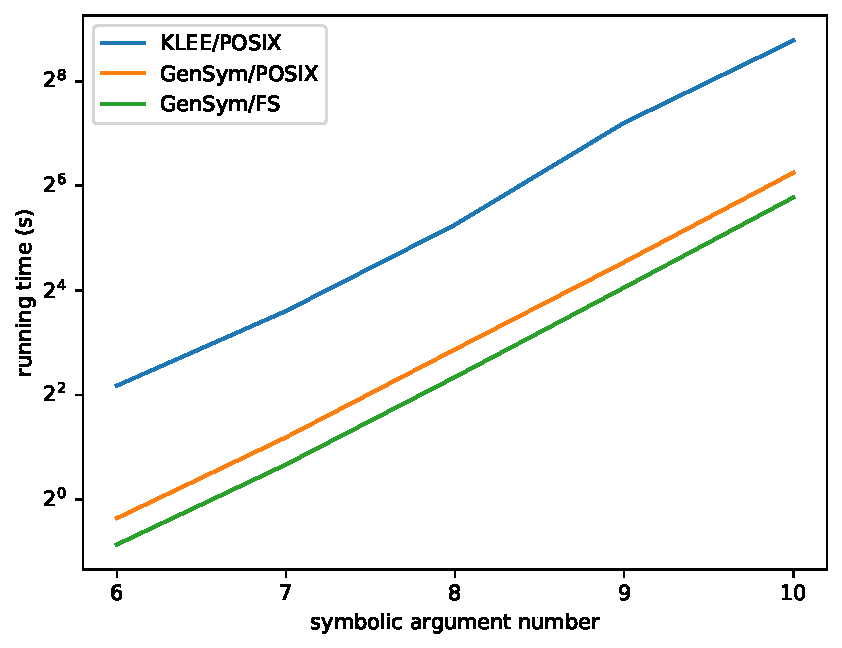
\includegraphics[scale=0.6]{evaluationplot.pdf}
  \caption{Running time of KLEE/POSIX, \tool/POSIX and \tool/FS}
  \label{fig:speedup}
\end{figure}
We first observe that KLEE/POSIX, \tool/POSIX and \tool/FS explore the same number of paths, this validate the correctness of our symbolic execution engine and our internal file system using KLEE as a reference. \par
The result demonstrates that our internal file system has faithfully modeled KLEE's POSIX file system. We can observe that our internal file system also performs better than KLEE's POSIX file system in our engine with a steady 1.4x speedup based on the comparison between \tool/FS and \tool/POSIX. This validate our observation in Section \ref{twofsimpl} that although implementing file system in the source language level has the benefit of flexibility and portability, it lacks performance and efficiency as the file system always executes on the control and memory abstraction of the underlying engine. Levels of indirection will cause a significant performance degrading.\par
Besides the comparison between the two file system implementations in \tool, the comparison between \tool/POSIX and KLEE/POSIX demonstrates that our framework really out performs KLEE. \tool achieves a 5x to 6x speedup over KLEE while analyzing the same program and obtaining the same path coverage. This speedup comes from two aspects, the eliminated interpretation overhead, and the optimization opportunity enabled by code generation. This proves our claim that we could realize efficient symbolic execution by adopting modern compilation and code generation techniques.
\section{Conclusion}\label{conclusion}
We discuss two different approaches of modeling environment in the context of symbolic execution compiler. Modern code generation techniques allow implementing the file system environment both at source language level an the target language level. The former approach is flexible and portable while the later approach has the advantage of performance and efficiency. We test Coreutils program as a benchmark for environment modeling in symbolic execution. We overcome several obstacles towards testing Coreutils and optimized the compilation time. The final Coreutils benchmark of both file system implementations in \tool and KLEE validates our claim and deepen our understanding of symbolic execution.
\bibliographystyle{acm}
\bibliography{paper}
\end{document}
\endinput
